\chapter{Non-parametric approximation of athe regression function}
\section{Introduction}
%The subject of the fifth laboratory class was a continuation of non-parametric approximation methods. 
%This time however, instead of having to use a trigonometric basis, we were free to chose basis ourselves. 

The subject of the fifth laboratory was approximation of a regression function using a rational function.
Given a regression function $R(u)$ we can rewrite it as  $R(u) = \frac{R(u)f(u)}{F(u)}$ and further $R(u) = \frac{g(u)}{f(u)}$ where, $g(u) = R(u)f(u)$, and  $f(u) - \text{p.d.f.}$. \\
On a given interval, every function can be defined uniquely as an infinite series in terms off an orthonormal basis:
\begin{equation}
    R(u) = \frac{g(u)}{f(u)} = \frac{\Sigma_{i=1}^{\infty}b_i\phi_i(u)}{ \Sigma_{i=1}^{\infty}a_i\phi_i(u)}
\end{equation}
Where:
\begin{itemize}
        \item $\phi_i$ - an orthonormal function possessing all the properties described in the previous report.
        \item $a_i = E\phi_I(u_k)$
        \item $b_i = E y_k\phi_I(u_k)$
\end{itemize}
We can use this definition to approximate the regression function as follows:
\begin{equation}
    \hat{R}(u) = \frac{\hat{g}(u)}{\hat{f}(u)} =   \frac{\Sigma_{i=1}^{S}\hat{b}_i\phi_i(u)}{ \Sigma_{i=1}^{S}\hat{a}_i\phi_i(u)}
\end{equation}
Where:
\begin{itemize}
        \item S - the amount of terms used for the approximation
        \item $\hat{a}_i = \frac{1}{N} \Sigma_{k=1}^{N}\phi_i(u_k)$
        \item $\hat{b}_i = \frac{1}{N} \Sigma_{k=1}^{N}y_k\phi_i(u_k)$
\end{itemize}
\\
The basis chosen were the Legendre's polynomials, which are orthogonal on the range of $x \in [-1,1]$.
They can be defined by the recurrence relation:
\begin{equation}
    nP_{n}(x) = (2n-1)xP_{n-1}(x) - (n-1)P_{n-2}(x)
\end{equation}
With:
\begin{itemize}
    \item $P_1(x)=1$
    \item $P_2(x) = x$
\end{itemize}

\begin{figure}[h!]
\begin{center}
\begin{tikzpicture}
\begin{axis}[
    xmin = -1, xmax = 1,
    ymin = -1.25, ymax = 1.25,
    grid = both,
    minor tick num = 1,
    major grid style = {lightgray},
    minor grid style = {lightgray!25},
    width = \textwidth,
    height = 0.5\textwidth,
    xlabel = x,
    ylabel = y]

    \addplot[color=blue,
        ]
        table [col sep=space, x index = 0, y index=1]{./plot_data/chapter_4/legendre.dat};

    \addplot[color=yellow,
        ]
        table [col sep=space, x index = 0, y index=2]{./plot_data/chapter_4/legendre.dat};

    \addplot[color=red,
        ]
        table [col sep=space, x index = 0, y index=3]{./plot_data/chapter_4/legendre.dat};

    \addplot[color=green,
        ]
        table [col sep=space, x index = 0, y index=4]{./plot_data/chapter_4/legendre.dat};

    \addplot[color=orange,
        ]
        table [col sep=space, x index = 0, y index=5]{./plot_data/chapter_4/legendre.dat};

    \legend{
        $P_0$,
        $P_1$,
        $P_2$,
        $P_3$,
        $P_4$}
\end{axis}
\end{tikzpicture}
\end{center}

\label{app_fig}
\caption{The first four Legendre polynomials}
\end{figure}



Note that these polynomials are merely orthogonal, for the purpose of non-parametric approximation we have to normalize them as follows:
\begin{equation}
    \mathcal{P}_n(x) = P_n(x)\sqrt{n-0.5}
\end{equation}

As before, we were divided into 2 groups, each of which had to approximate one of the 2 functions plotted below:



\begin{figure}[h!]
\begin{center}
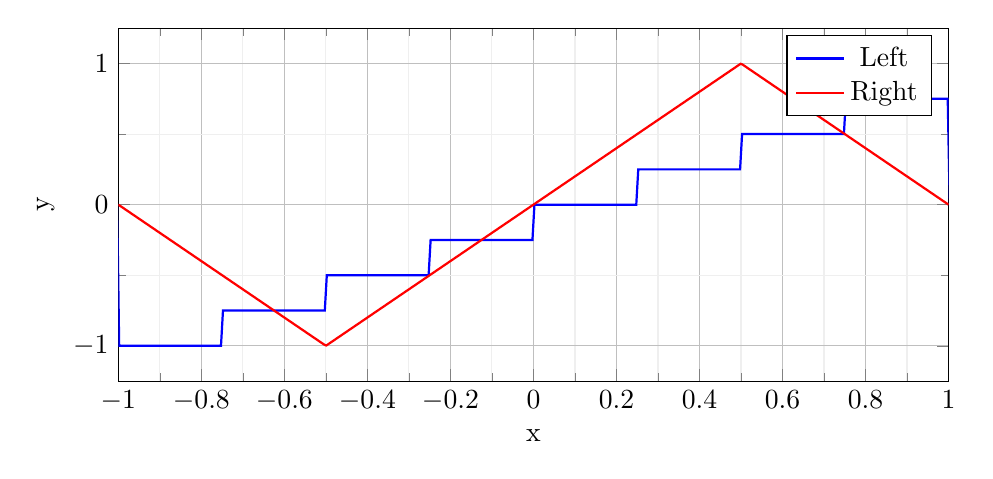
\begin{tikzpicture}
\begin{axis}[
    xmin = -1, xmax = 1,
    ymin = -1.25, ymax = 1.25,
    grid = both,
    minor tick num = 1,
    major grid style = {lightgray},
    minor grid style = {lightgray!25},
    width = \textwidth,
    height = 0.5\textwidth,
    xlabel = x,
    ylabel = y]

    \addplot[
        domain = -1.2:1.2,
        samples = 500,
        thick,
        blue,
        ] 
        {
        (x > -1)*(x < 1)*(floor(4*x)/4)
        };


    \addplot[
        domain = -1:1,
        samples = 500,
        thick,
        red,
        ] 
        {
        (x > -0.5)*(x < 0.5)*(2*x) + (x < -0.5)*(-2*x-2)   + (x > 0.5)*(-2*x+2)
        };





    \legend{
        Left,
        Right,
        }
\end{axis}
\end{tikzpicture}
\end{center}

\label{app_fig}
\caption{The first four Legendre polynomials}
\end{figure}




\section{Laboratory}
Several such approximations can be seen below superimposed with the original function:

%%

For the triangle function this approximation works very well. Oneo f the reasons for this, is that the values of the approximated function at the borders of the interval of approximation are equal to 0. For the other funciton, we can observe how divverent values at the boundry introduce an error.
%%%

\section{Conclusions}
For certain functions these rational approximations work very well, for others not so much. One of the reasons for the use of 

